\chapter{Wirtualizacja systemów operacyjnych}

\begin{figure}[ht]
    \centering
    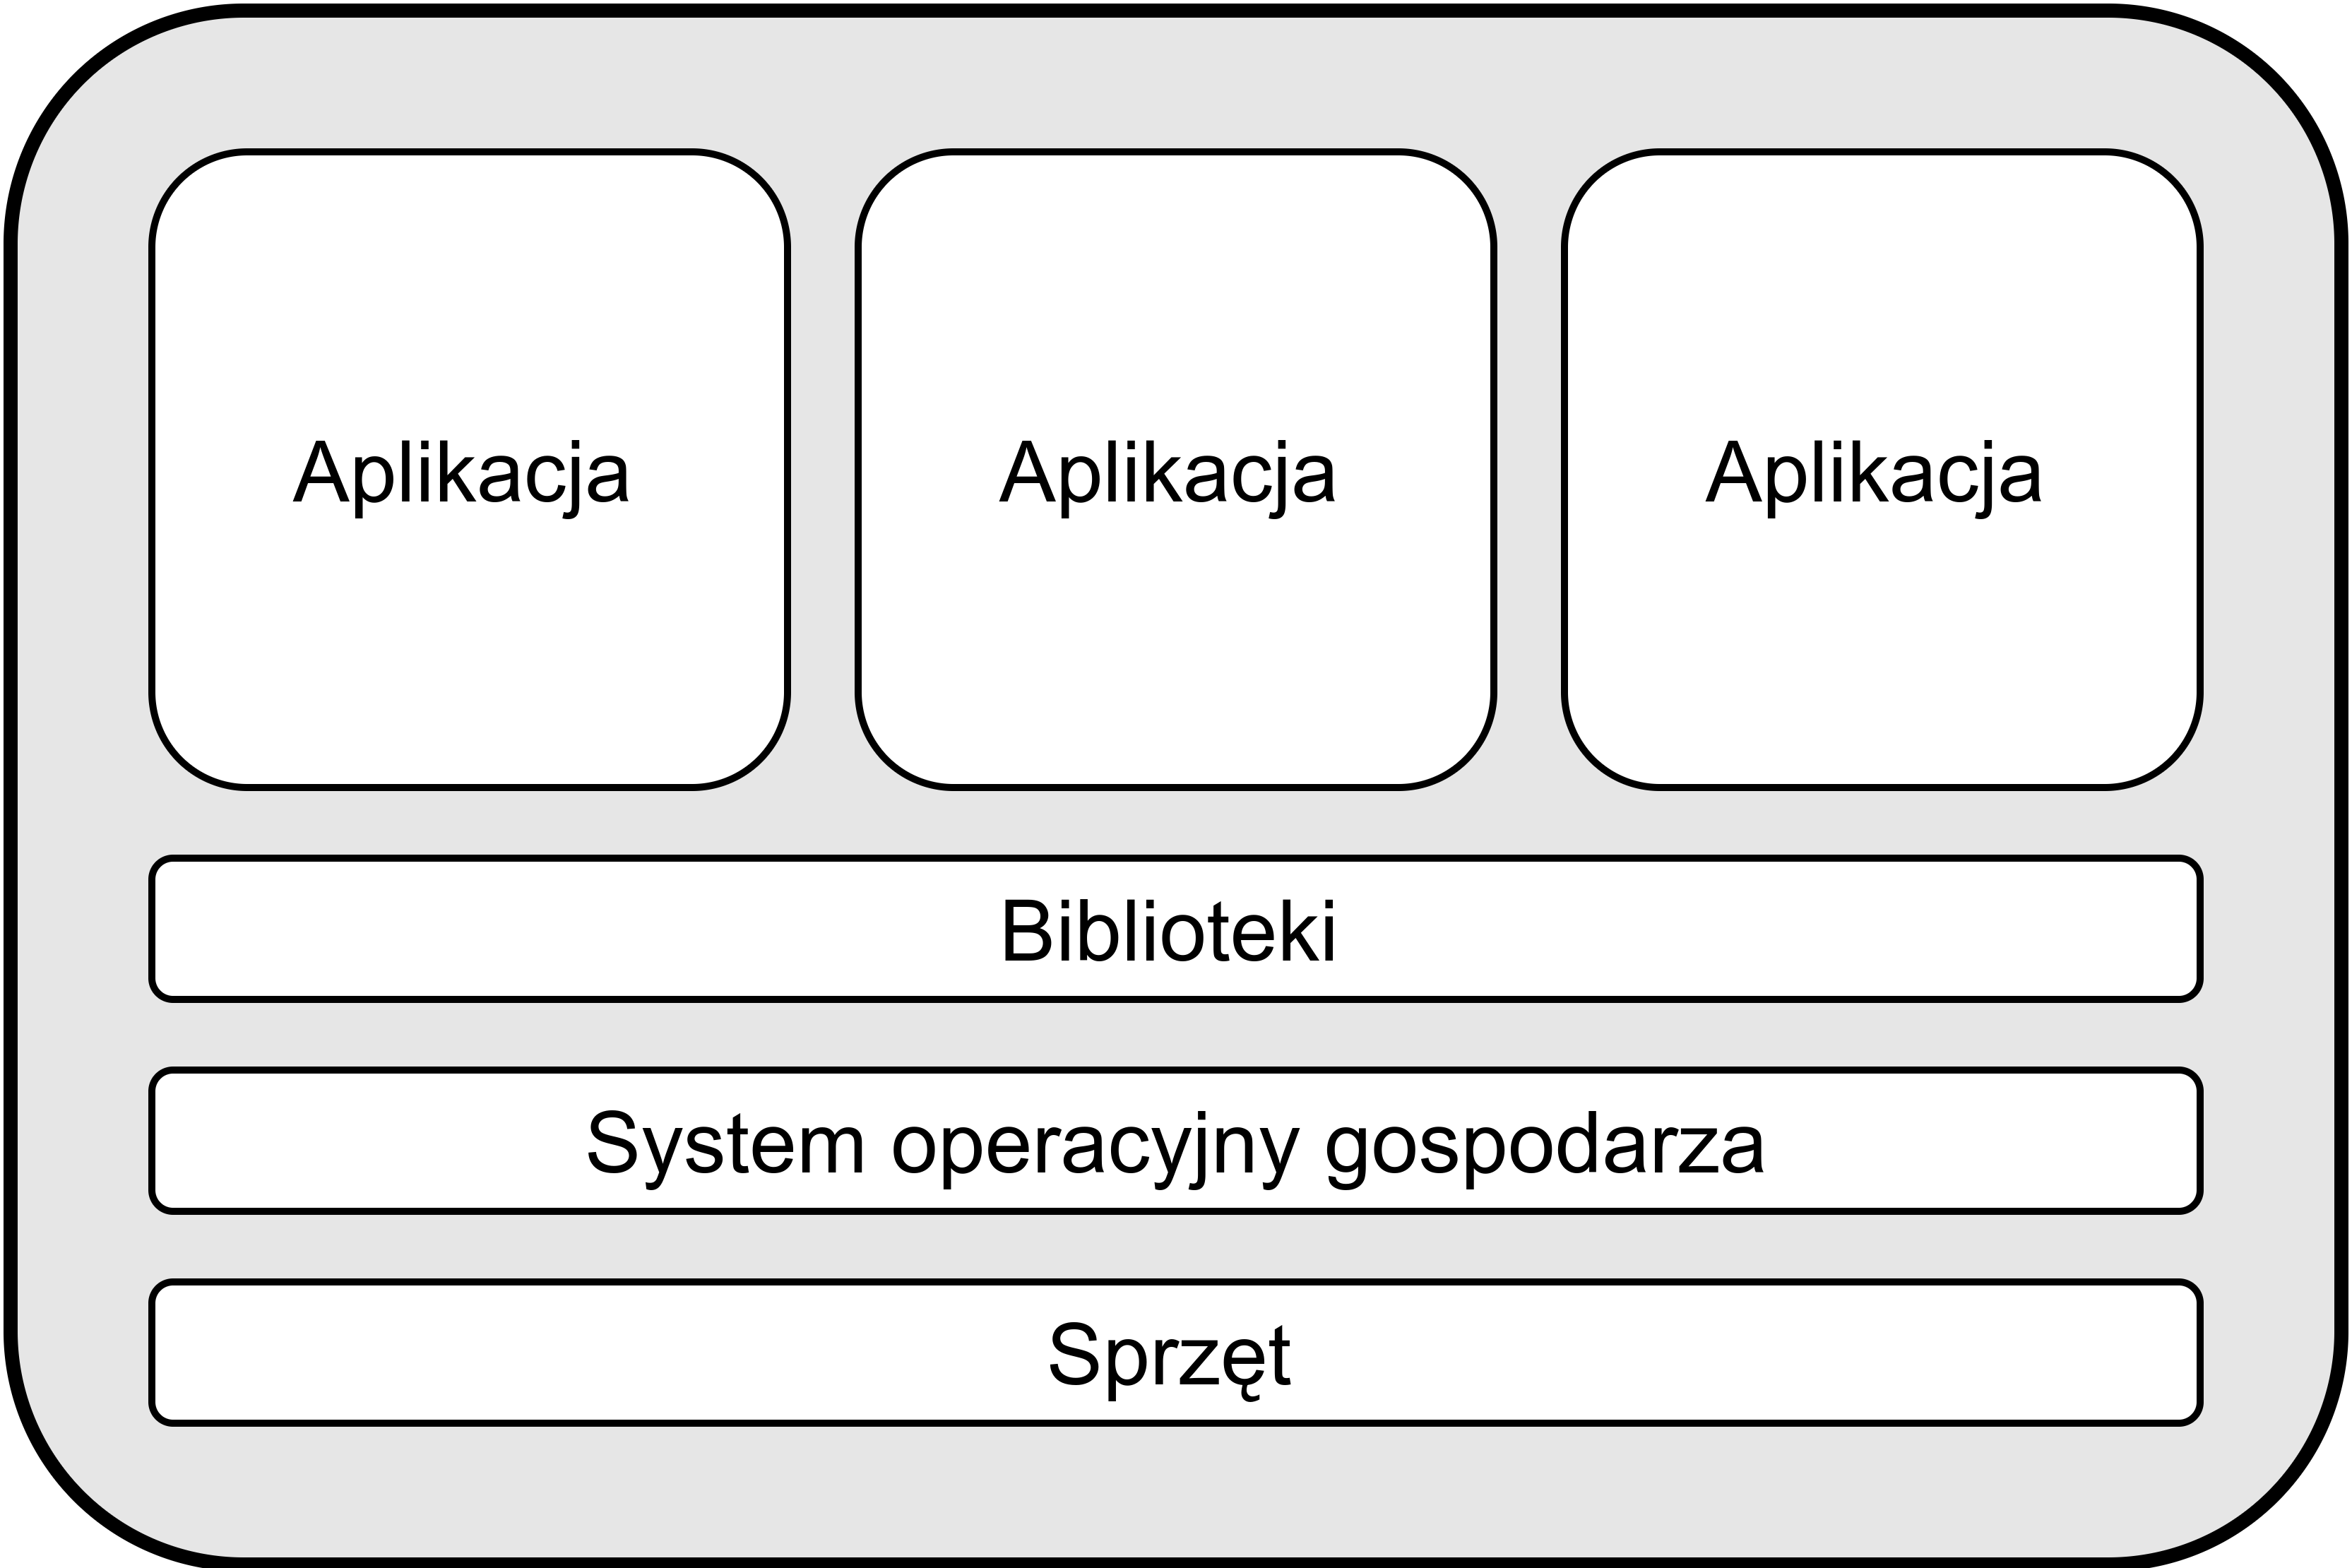
\includegraphics[width=0.45\linewidth]{images/native.png}
    \caption{Schemat infrastruktury uruchomionej natywnie}
    \label{fig:native}
\end{figure}

Rozdział ten przedstawia dostepne rozwiązania wirtualizacji systemów operacyjnych. Zastosowania chmurowe zwykle wykorzystują wirtualizację jako element zabezpieczeń, umożliwiając łatwiejsze zarządzanie bezpieczeństwem złożonego klastra lub infratruktury chmurowej. Poprawnie skonfigurowana architektura usprawnia monitorowanie poprawności systemu gościa i~warstwy wirtualizacji oraz chroni je przed większością rodzajów ataków, zachowując jednocześnie pełną przejrzystość dla dostawcy i~użytkownika usługi. Co więcej, pozwala na lokalne reagowanie na naruszenia bezpieczeństwa oraz powiadamianie o~takich wydarzeniach.

Możliwe jest także stworzenie architektury chmurowej całkowicie w~oparciu o~rozwiązania Open Source. Wyniki analiz pokazują, że takie podejście są skuteczne, a~kompromis pomiędzy wydajnością i~bezpieczeństwem akceptowalny \cite{LombardiSecureVirtualizationOfCloudComputing}. Jednakże, biorąc pod uwagę pewne podstawowe ograniczenia, takie jak narzut wydajności, elastyczność i~skalowalność, pojawiły się alternatywne rozwiązania dla wirtualizacji w~postaci kontenerów i~unikerneli.

\section{Maszyny wirtualne}

\begin{figure}[ht]
    \begin{subfigure}{0.5\textwidth}
        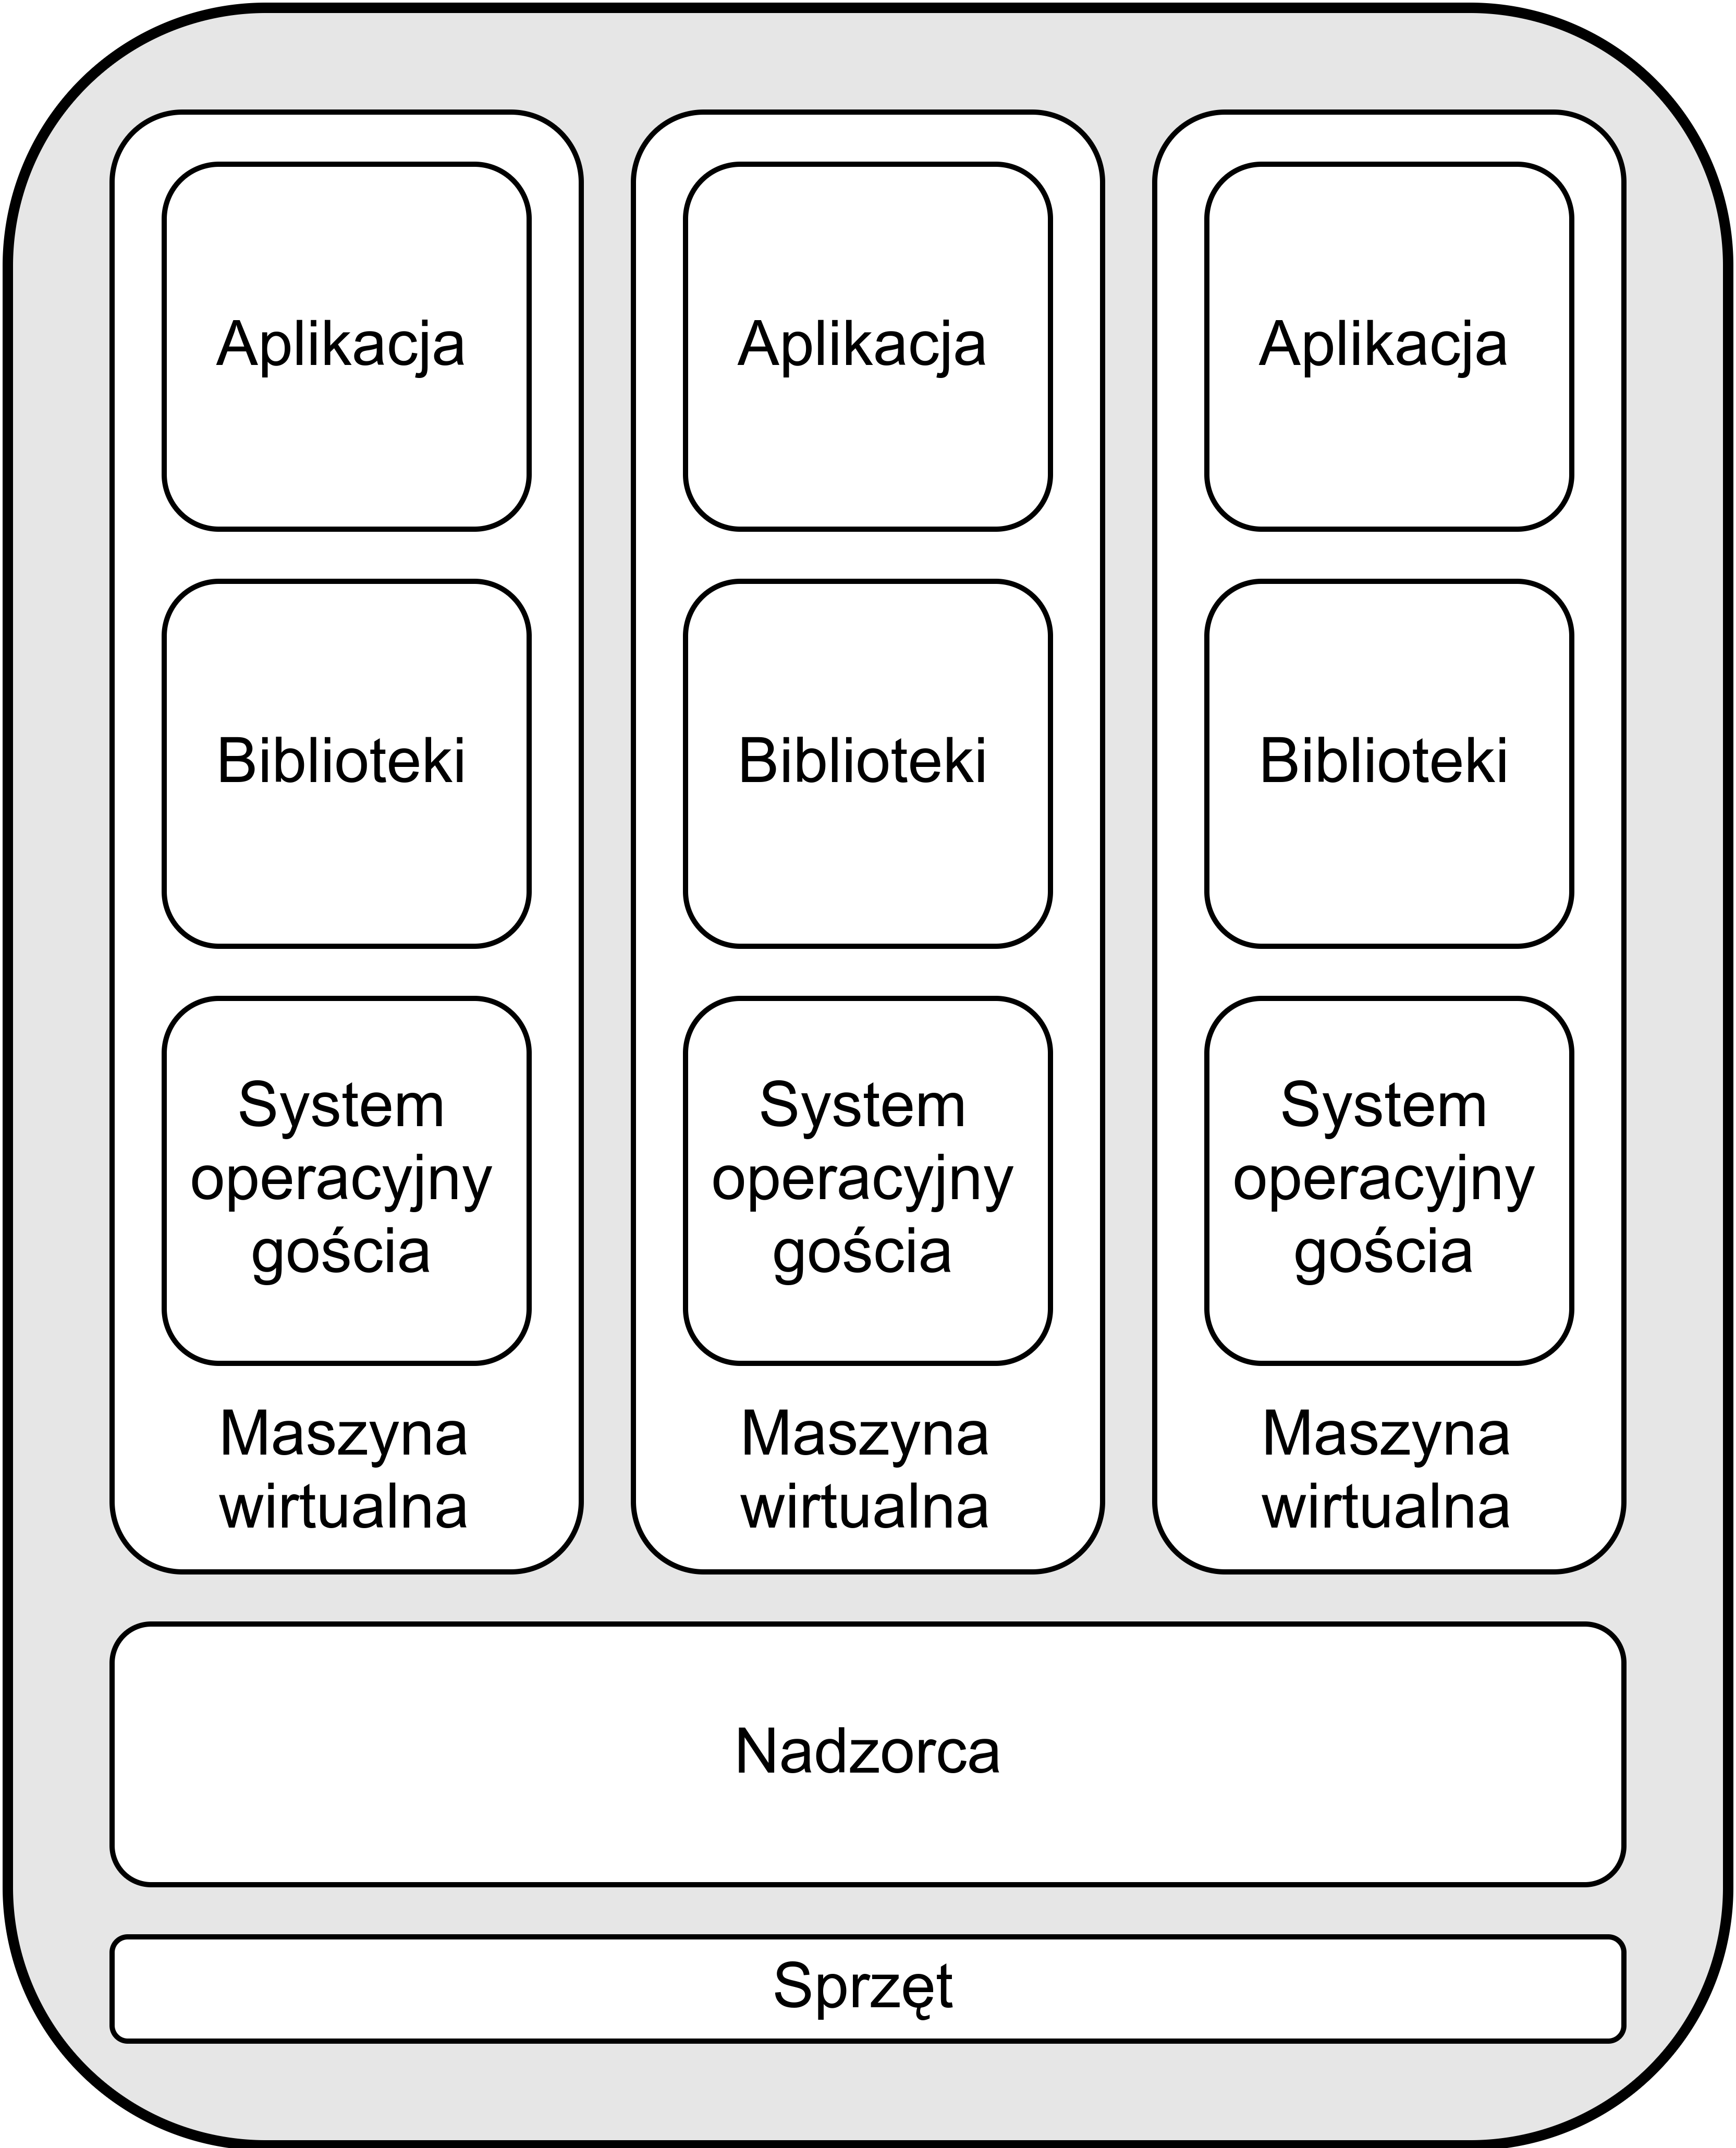
\includegraphics[width=0.9\linewidth]{images/hardwareVM.png}
        \caption{bezpośrednio na sprzęcie}
        \label{fig:hardwareVM}
    \end{subfigure}
    \begin{subfigure}{0.5\textwidth}
        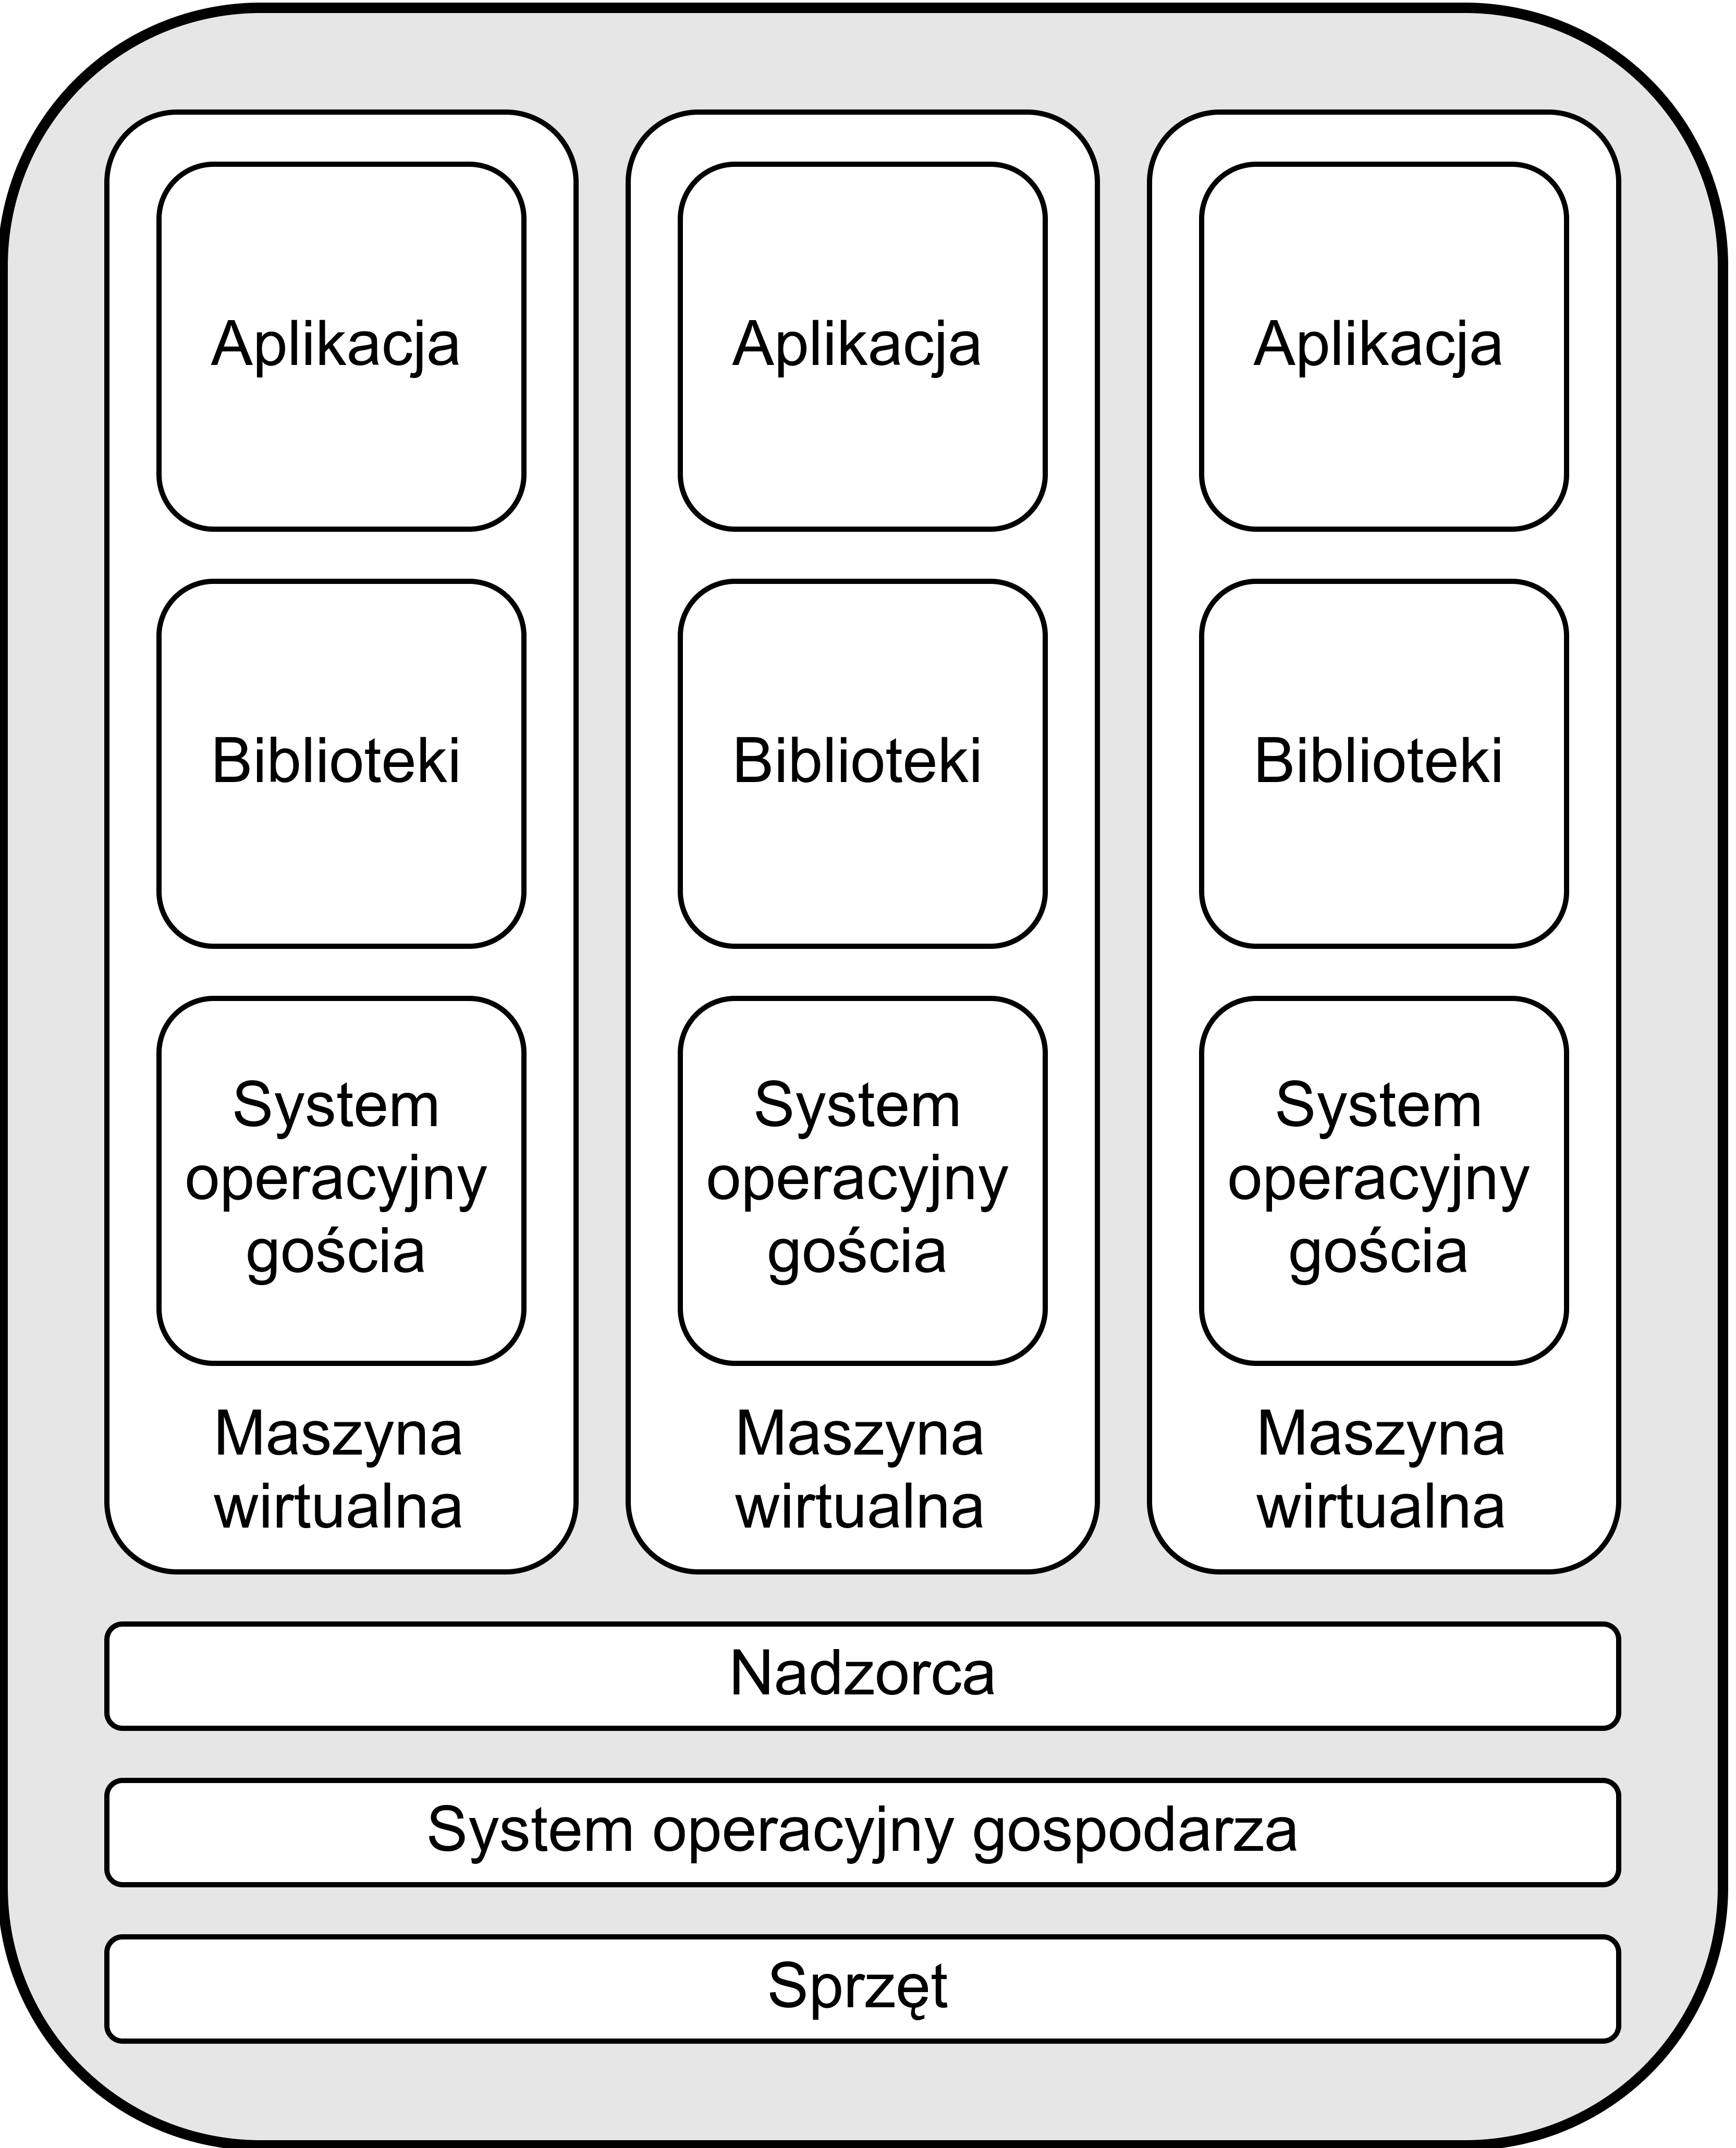
\includegraphics[width=0.9\linewidth]{images/OSVM.png}
        \caption{na systemie operacyjnym gospodarza}
        \label{fig:OSVM}
    \end{subfigure}
    \caption{Schemat infrastruktury uruchomionej na maszynach wirtualnych z~nadzorcą}
    \label{fig:VMs}
\end{figure}

Maszyny wirtualne są najczęstszym sposobem wirtualizacji przetwarzania w~chmurze: są w~pełni funkcjonalnym systemem operacyjnym, działającym na emulowanej warstwie sprzętowej, zapewnianej przez leżącego u~podstaw nadzorcę. Nadzorca może działać bezpośrednio na sprzęcie (np.~Xen)(rys.~\ref{fig:hardwareVM}) lub na systemie operacyjnym gospodarza (np.~KVM)(rys.~\ref{fig:OSVM}). Maszynę wirtualną można klonować, instalować w~ciągu kilku minut i~uruchamiać w~ciągu kilku sekund, co pozwala na tworzenie całego stosu technologicznego za pomocą scentralizowanych narzędzi. Jednak obecność dwóch systemów operacyjnych (gospodarza i~gościa) wraz z~dodatkową, wirtualną warstwą sprzętową wprowadza znaczne narzuty w~wydajności. Sprzętowa obsługa wirtualizacji radykalnie zmniejsza przytoczony narzut, ale wydajność jest daleka od operowania bezpośrednio na sprzęcie, szczególnie w~przypadku operacji wejścia/wyjścia.

Wyniki badań wyraźnie pokazują, że wydajność nadzorcy działającego na systemie operacyjnym gospodarza znacznie się poprawiła w~ciągu ostatnich kilku lat. Niemniej jednak szczególnie wydajność operacji na dysku twardym może nadal stanowić wąskie gardło w~przypadku niektórych rodzajów aplikacji \cite{MorabitoHypervisorsVSLightweightVirtualization}.

Podobna sytuacja dotyczy nadzorcy działającego bezpośrednio na sprzęcie. W~jego przypadku za słabą wydajność operacji na dysku odpowiadają parasterowniki, które pomimo wielu usprawnień wprowadzanych od kilku lat nie są w~stanie osiągnąć wyników zbliżonych do innych rozwiązań \cite{XavierPerformanceEvaluationOfContainerBasedVirtualizationForHighPerformanceComputingEnvironments}.

\section{Kontenery}

\begin{figure}[ht]
    \centering
    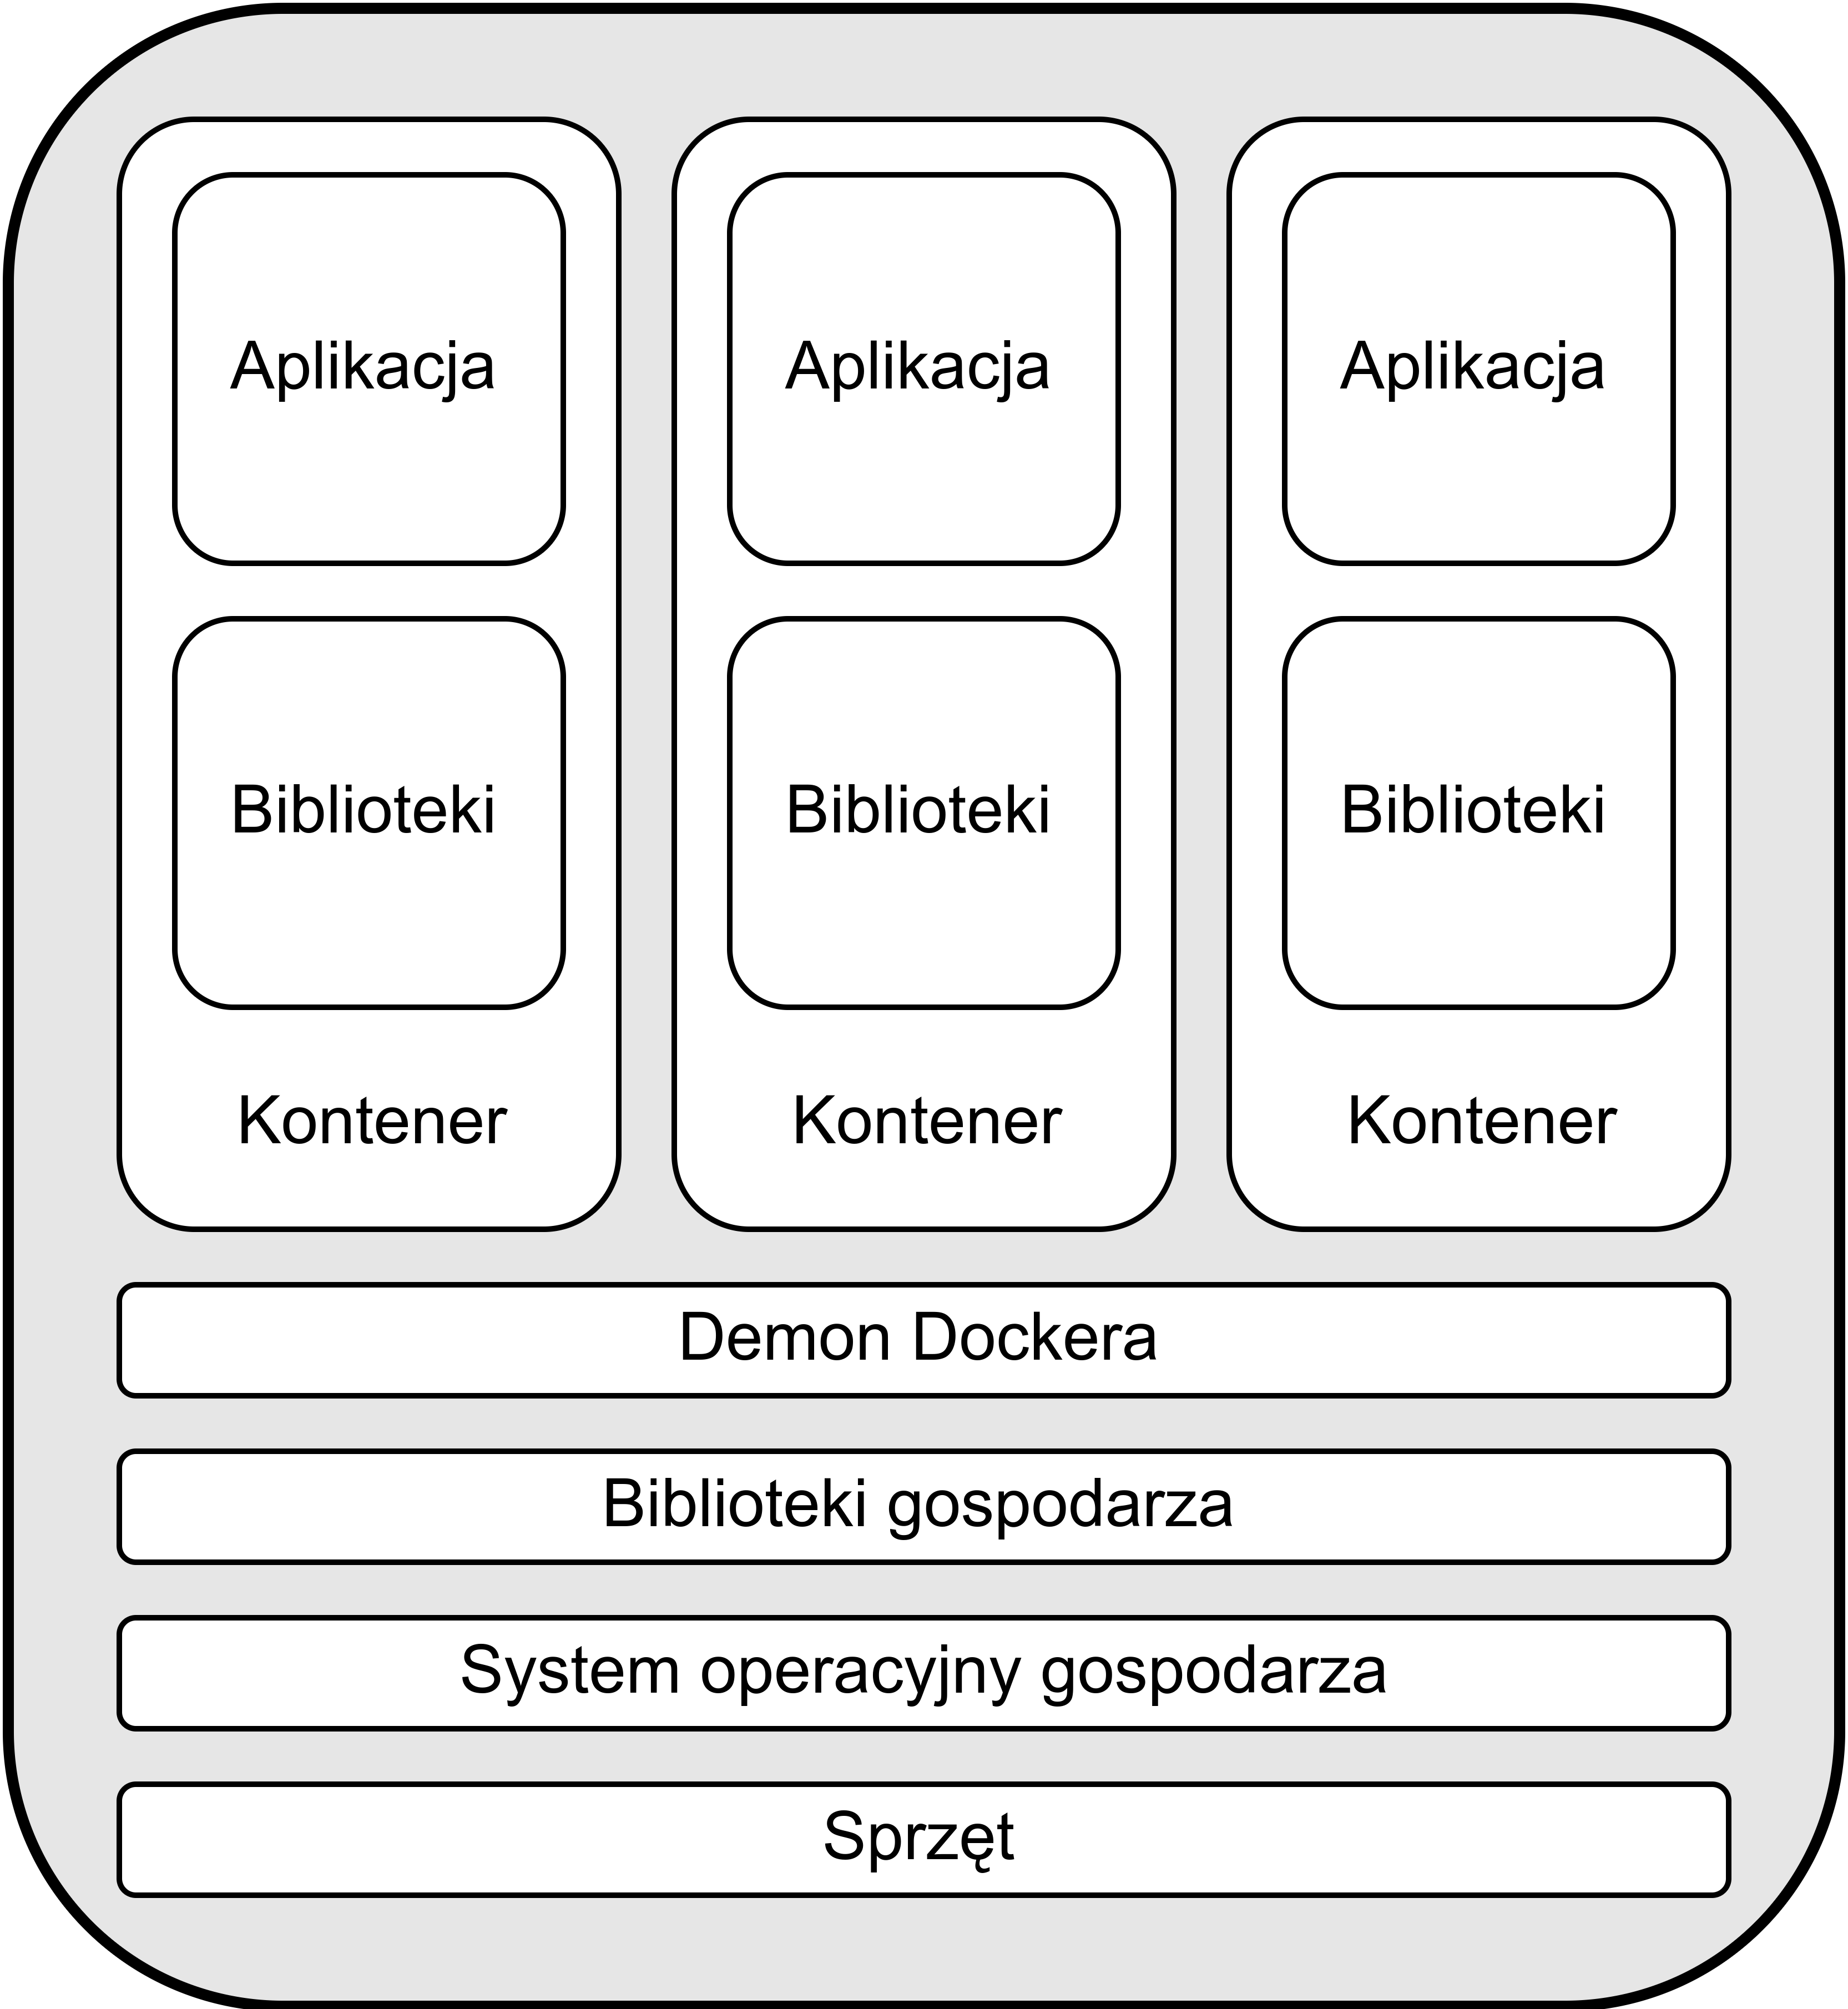
\includegraphics[width=0.45\linewidth]{images/container.png}
    \caption{Schemat infrastruktury uruchomionej na kontenerach}
    \label{fig:container}
\end{figure}

Kontenery (rys.~\ref{fig:container}) zapewniają prawie, że natywną wydajność w~przeciwieństwie do wirtualizacji \cite{MorabitoHypervisorsVSLightweightVirtualization}\cite{XavierPerformanceEvaluationOfContainerBasedVirtualizationForHighPerformanceComputingEnvironments} z~dodatkową możliwością płynnego uruchamiania wielu aplikacji na tej samej maszynie. Nowe instancje kontenerów można tworzyć niemal natychmiastowo aby sprostać szczytowi zapotrzebowania klientów. Kontenery istniały od dawna w~różnych formach, które różnią się poziomem zapewnianej izolacji. Na przykład, \textit{BSD~jails} \cite{KampJails} i~\textit{chroot} można uznać za wczesną formę technologii kontenerowej. Najnowsze rozwiązania kontenerowe oparte na systemie Linux, bazują w~dużej mierze na wsparciu jądra, bibliotece przestrzeni użytkownika zapewniającej interfejs do wywołań systemowych i~aplikacji dla użytkownika rozwiązania kontenerowego. Istnieją dwie główne implementacje kontenerów: implementacja oparta na LXC, z~wykorzystaniem narzędzi \textit{cgroups} i~\textit{namespaces} oraz łatka jądra o~nazwie OpenVZ. Spis poszczególnych technologii kontenerowych przedstawia tabela~\ref{table:containers}.

\begin{table}[ht]
    \begin{tabular}{|L{2.3cm}|L{1.8cm}|L{2.5cm}|L{3.5cm}|L{4.5cm}|}
        \hline
        \textbf{Technologia} & \textbf{Podstawa} & \textbf{Biblioteka} & \textbf{Zależności jądra} & \textbf{Dodatkowe zależności} \\
        \hline
        LXC & LXC & liblxc & cgroups, namespaces, capabilities & golang \\
        \hline
        LXD & LXC & liblxc & cgroups, namespaces, capabilities & LXC, golang \\
        \hline
        Docker & LXC & libcontainer & cgroups, namespaces, capabilities, kernel w~wersji 3.10+ & iptables, perl, AppArmor, sqlite, golang \\
        \hline
        Rocket & LXC & AppContainer & cgroups, namespaces, capabilities, kernel w~wersji 3.8+ & cpio, golang, squashfs, gpg \\
        \hline
        Warden & LXC & \textit{brak} & cgroups, namespaces & debootstrap, rake \\
        \hline
        OpenVZ & OpenVZ & libCT & niestandardowa aktualizacja jądra & specific components: CRIU, ploop, VCMMD \\
        \hline
    \end{tabular}
    \caption{Rozwiązania kontenerowe}
    \label{table:containers}
\end{table}

Kontenery można wykorzystać w~środowisku wielu dzierżawców (ang. multi-tenant environment), wykorzystując w~ten sposób współdzielenie zasobów w~celu zwiększenia średniego zużycia sprzętu. Cel ten osiąga się poprzez współdzielenie jądra z~maszyną gospodarza. W~przeciwieństwie do maszyn wirtualnych, kontenery nie uruchamiają własnego jądra, ale działają bezpośrednio na jądrze gospodarza. Skraca to ścieżkę wykonywania wywołań systemowych poprzez usunięcie warstwy jądra gościa i~wirtualnej warstwy sprzętowej. Dodatkowo, kontenery mogą współdzielić zasoby oprogramowania (np.~biblioteki) z~gospodarzem, unikając powielania kodu. Brak dodatkowego jądra i~niektórych bibliotek systemowych (udostępnianych przez gospodarza) sprawia, że kontenery są bardzo lekkie (rozmiary obrazów mogą się zmniejszyć do kilku megabajtów). Dzięki temu proces uruchamiania jest bardzo szybki (nawet poniżej jednej sekundy \cite{ZhengIntegratingContainersIntoWorkflows}).

Pozwala to na ponowne uruchamianie kontenerów na żądanie lub szybkie ich przenoszenie. Jak pokazują niektóre przykłady zastosowań technologii kontenerowych możliwe jest tworzenie aplikacji, które dynamicznie uruchamiają i~usuwają kontenery wykorzystywane do wykonywania krótkich zadań. Wydajność takiego rozwiązania jest jednak ograniczona i~przy systemach wykorzystujących tysiące kontenerów koszty abstrakcji zaczynają być wyższe niż zyski wynikające z~tak rozproszonej architektury \cite{ZhengIntegratingContainersIntoWorkflows}.

Działanie wielu takich kontenerów -- domyślnie nieświadomych siebie nawzajem pomimo współużytkowania jądra gospodarza -- wymaga jednak dodatkowej izolacji. Popularność Dockera jako jednego z~przykładów rozwiązania kontenerowego, w~połączeniu z~rozszerzonymi uprawnieniami na uruchamianych maszynach, czyni go celem o~wysokiej wartości dla atakującego. Dlatego też w~kolejnych rozdziałach praca koncentruje się na podatnościach, na które jest narażony, i~możliwych środkach zaradczych.

\section{Unikernele}

\begin{figure}[ht]
    \centering
    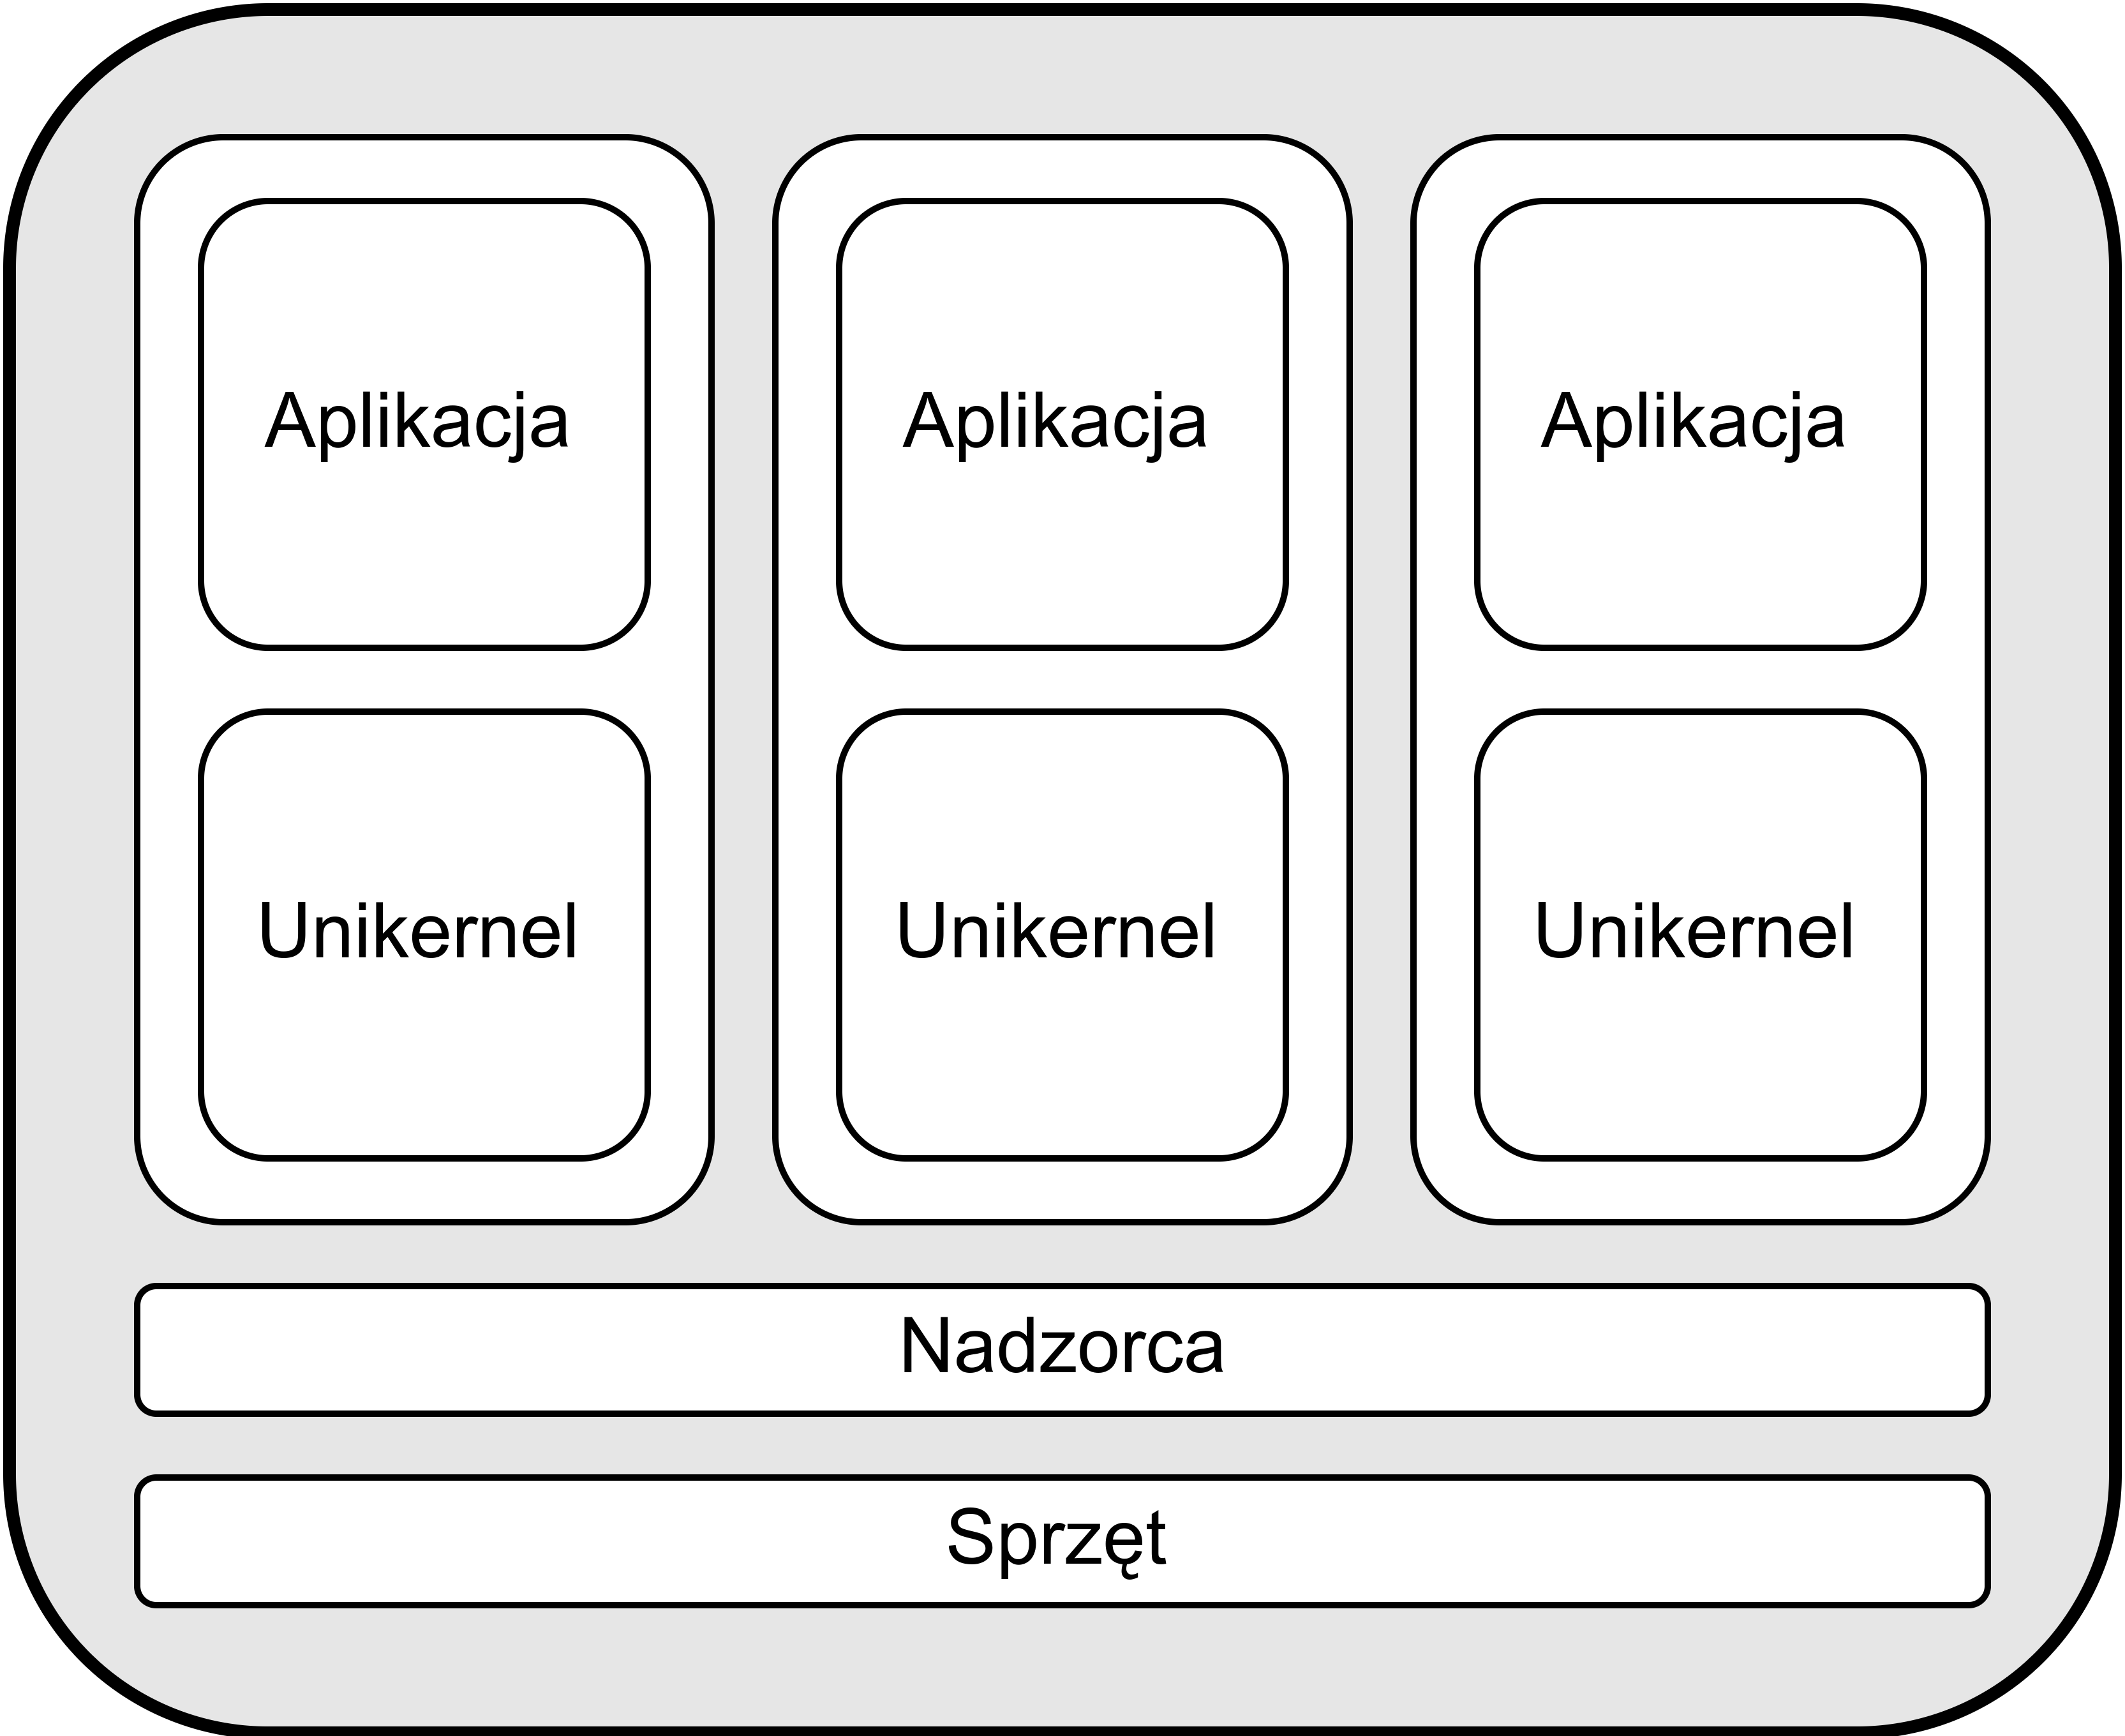
\includegraphics[width=0.45\linewidth]{images/unikernel.png}
    \caption{Schemat infrastruktury uruchomionej na unikernelach}
    \label{fig:unikernel}
\end{figure}

Unikernele (rys.~\ref{fig:unikernel}) składają się z~bardzo lekkich systemów operacyjnych, specjalnie zaprojektowanych do działania na maszynie wirtualnej. Unikernele zostały pierwotnie zaprojektowane do działania na nadzorcy Xen. Są bardziej wydajne niż klasyczna maszyna wirtualna gdyż skracają ścieżkę wykonywania wywołań systemowych: nie korzystają z~ parasterowników, a~nadzorca nie emuluje warstwy sprzętowej. Interakcję osiąga się za pomocą specjalnego interfejsu programistycznego. Umożliwia on optymalizacje, które były niemożliwe w~przypadku starszego modelu maszyn wirtualnych, gdzie niezmodyfikowane jądro działało na emulowanym sprzęcie. Jednakże, te modyfikacje uzależniają unikernele od nadzorcy, na którym działają.

W chwili obecnej większość rozwoju unikerneli jest związana z~nadzorcą Xen. Ponadto, unikernele są zwykle zaprojektowane do uruchamiania programów napisanych w~określonym języku programowania. W~związku z~tym osadzają one tylko biblioteki potrzebne dla konkretnego języka i~pod niego są zoptymalizowane (np.~HaLVM dla Haskell, OSv dla Java, C, C++, Ruby i~Node.js, LING dla Erlang). Wszystkie powyższe zmiany zmniejszają narzut w~stosunku do maszyn wirtualnych \cite{XenWiki}.

Wyniki analiz pokazują, że unikernele w~rzeczywistości osiągają lepszą wydajność niż maszyny wirtualne, a~ponadto rozwiązują niektóre problemy związane z~bezpieczeństwem, na jakie narażone są kontenery. Zalety dotyczące bezpieczeństwa wynikają z~tego, że aplikacje działające w~unikernelach nie współużytkują jądra systemu operacyjnego. Badania stwierdzają, że implementacje unikerneli nie są wystarczająco dojrzałe, aby można je było szeroko rozpowszechnić w~produkcji. Próby stworzenia środowisk produkcyjnych wymagały dużej ilość optymalizacji pod konkretne rozwiązania, a~brak porządnych narzędzi deweloperskich znacznie wydłużał czas rozwoju. Uważa się jednak unikernele za poważnych konkurentów dla kontenerów w~dłuższej perspektywie czasu, zarówno ze względów bezpieczeństwa, jak i~ze względu na ich bardzo krótki czas uruchamiania \cite{KuenzerUnikernelsEverywhere}\cite{MadhavapeddyUnikernels}.

Unikernele mogą w przyszłości oferować znaczne korzyści dla użytkowników biznesowych, którzy z reguły starają się zmniejszać koszty poprzez minimalne wydatki na rozwiązania bezpieczeństwa i prywatności danych. Unikernele poprzez swoją idempotentość działania ograniczają liczbę błędów wykonywanych przez deweloperów, a tym samym łagodzą koszty deweloperskie. Ponadto, dzięki redukcji narzutów wirtualizacji pozwalają na lepsze wykorzystanie zasobów, prowadząc do jeszcze większych oszczędności w obszarze infrastruktury \cite{DuncanCloudCyberSecurity}.

\section{Porównanie}

Każda z~powyższych alternatyw zapewnia inny kompromis pomiędzy wieloma czynnikami: wydajnością, izolacją, czasem rozruchu, przestrzenią dyskową, zależnością od systemu operacyjnego i~dojrzałością. Większość z~tych czynników jest związana z~wydajnością, ale w~grę wchodzi również bezpieczeństwo i~dojrzałość rozwiązań. Zgodnie ze względnym znaczeniem tych parametrów i~zależnie od zamierzonego zastosowania każda z~alternatyw może być poprawnym wyborem.

Z jednej strony tradycyjne maszyny wirtualne pochłaniają dużo zasobów, a~ich uruchamianie i~wdrażanie przebiega wolno. Zapewniają jednak silną izolację, której doświadczono w~produkcji od wielu lat. Z~drugiej strony, kontenery są lekkie, bardzo szybkie we wdrożeniu i~rozruchu oraz, zmniejszając izolację, nakładają mniejszy narzut. Unikernele starają się osiągnąć kompromis między maszynami wirtualnymi, a~kontenerami, zapewniając szybkie i~lekkie środowisko wykonawcze działające na nadzorcy. Nadal jest to jednak rozwiązanie eksperymentalne. 

Dalsza część pracy skupia się wyłącznie na kontenerach jako obecnie najpopularniejszym rozwiązaniu wirtualizacji systemów operacyjnych.
